\chapter{BlenderSim}

\label{Chapter5}

\section{Overview}

%\todo{Add something about comparing the physics based motion to the real robot.}

Over the course of three months, a Blender based simulation was developed for HRTeam\footnote{HRTeam is a human and robot multi-agent framework developed to explore human and robot teamwork interactions \cite{hrteam}.} titled BlenderSim. Initially, BlenderSim was wholly physics based but soon proved to be problematic on three fronts: time, scale, and intricacy. The problems faced by using the physics engine to model the locomotion of the robots gave way to the thesis of tuning the physics engine via a genetic algorithm. In the interim, the physics engine was abandoned and a constant linear motion model was used. 

As a proof-of-concept of the thesis, BlenderSim was revisited with the physics engine being restored as the motion model---using the highest-fitness physics parameters found by BBAutoTune. Using only one robot, instead of the standard four usually used in a HRTeam experiment, the motion of the simulated, physics-based robot was compared to the real robot by re-running a previously run HRTeam experiment in BlenderSim.      

%Once BBAutoTune learned the physics engine parameters, the motion of the real robot, BlenderSim was restored to being wholly physics based with the physics engine modeling the locomotion of the real robots.


\section{Problems Faced}

Initial problems arose when the treads of the SRV-1 were recreated in the simulation. Even after numerous hours adjusting physics parameters and rigid-body configurations, the treads would consistently behave in erratic fashions. See Figure \ref{treads}.

\begin{figure}[htbp]
\centering
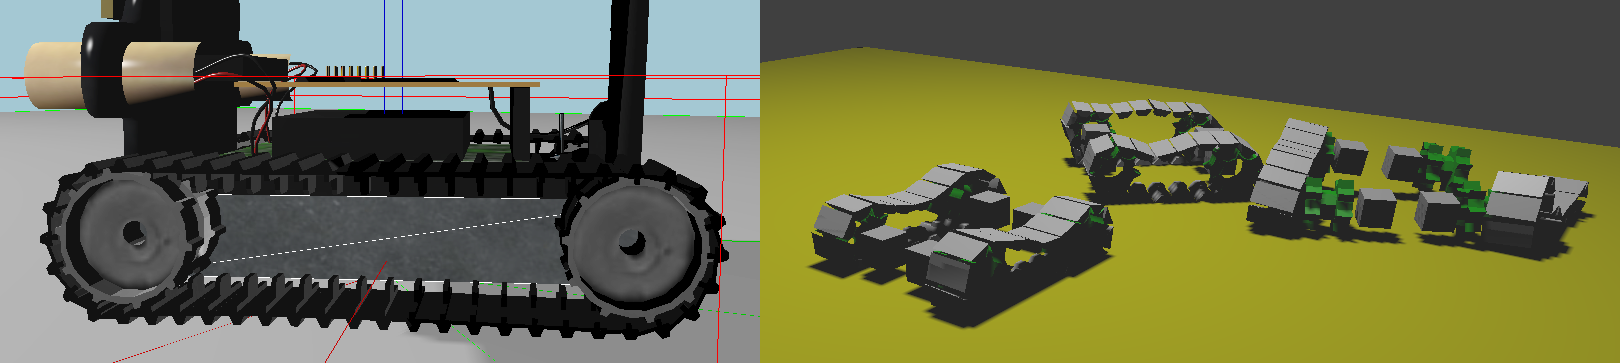
\includegraphics[scale=0.25]{../Figures/Chapter5/treads.png}
\rule{35em}{0.5pt}
\caption[Simulated Treads]{Here you see the to-scale treads modeled after the physical SRV-1 robot on the left and the physics-based rigid-body tracks in motion on the right.}
\label{treads}
\end{figure}

Scale was problematic as the Blender/Bullet physics engine has difficulty with collisions of objects that have a size outside of the assumed range of .05 to 10 meters \cite{website:bulletscale}. Objects smaller than .05 (5cm) Blender/Bullet units, in any given dimension, erratically jitter despite having no force acting upon them. 
%For instance, the wheels on the 3D SRV-1 model which are 2.11cm x 2.45cm x 2.52cm.
As such, since the wheel dimensions of the real SRV-1 are 2.11cm x 2.45cm x 2.52cm, the to-scale 3D model of the SRV-1 was affected by this scale limitation of the physics engine.

To rectify these issues, the physics engine was largely abandoned---in terms of providing the motion model---and was only kept to keep the robots from running through each other and the arena. In its place, a constant linear and angular velocity motion model was developed of which only moves the 3D robot as if it was a single point body. See Figure \ref{blendersimrun} and Figure \ref{sklarplots}. 

\begin{figure}[htbp]
\centering
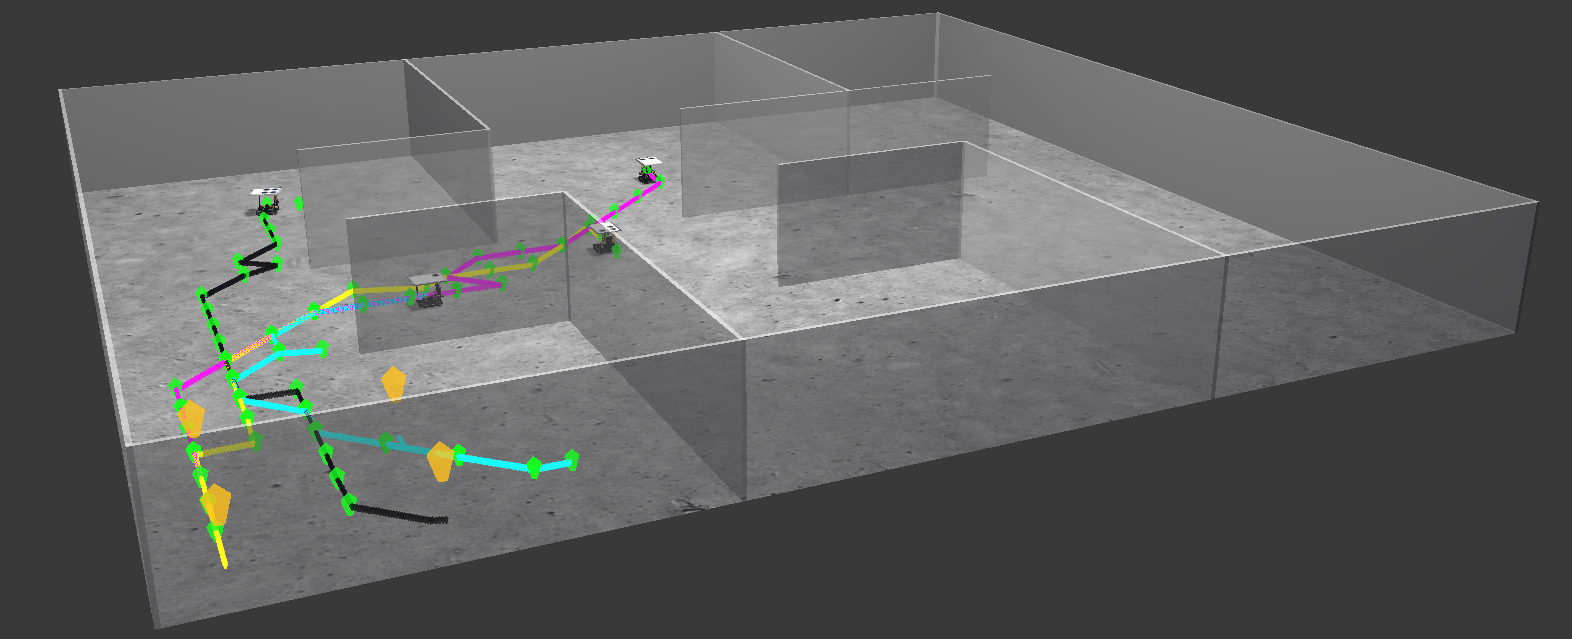
\includegraphics[scale=0.28]{../Figures/Chapter5/const_motion_model.png}
\rule{35em}{0.5pt}
\caption[Constant Velocity Locomotion Model]{Here you see the constant velocity motion model at work in BlenderSim with four robots traversing their respective paths of which consist of way-points scrapped from a previously recorded physical lab experiment.}
\label{blendersimrun}
\end{figure}

\begin{figure}[htbp]
\centering
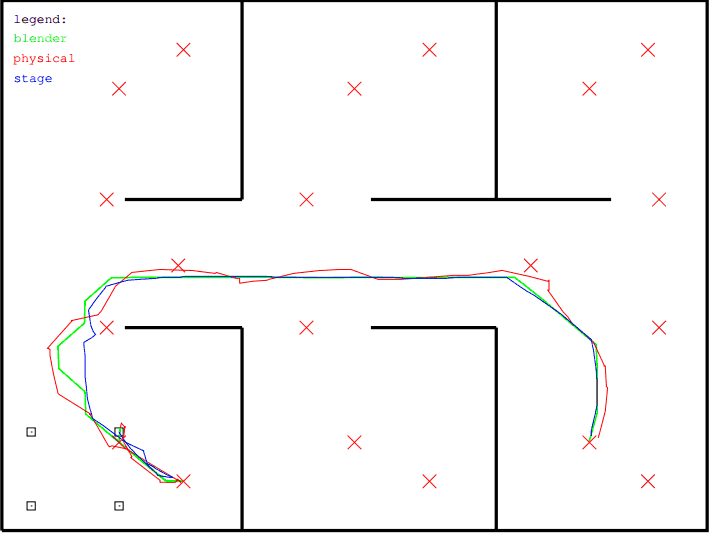
\includegraphics[scale=0.55]{../Figures/Chapter5/const_motion_model_plotted.png}
\rule{35em}{0.5pt}
\caption[Comparative Path Plots]{Here you see the path plots--as plotted by Dr. Elizabeth Sklar--of the BlenderSim robot, the physical robot, and the \textit{Stage} (a 2D robot simulator already in use by HRTeam)\cite{website:stage} robot plotted in comparison.}
\label{sklarplots}
\end{figure}

\section{Implementation}

For the purposes of the proof-of-concept, most of the original architecture of BlenderSim was simplified. The simulation contained one robot, one robot controller, one robot path planner, and the arena. 

\subsection{Arena}

The arena is a $602cm\times538cm$ enclosure with a main hallway and six compartments. The floor and all of walls are physics based in BlenderSim and respond accordingly should any robot try to pass through them. See Figure \ref{fig:arena_map}. All dimensions and proportions of the simulated arena match the real arena used in HRTeam experiments. 

\begin{figure}[htbp]
\centering
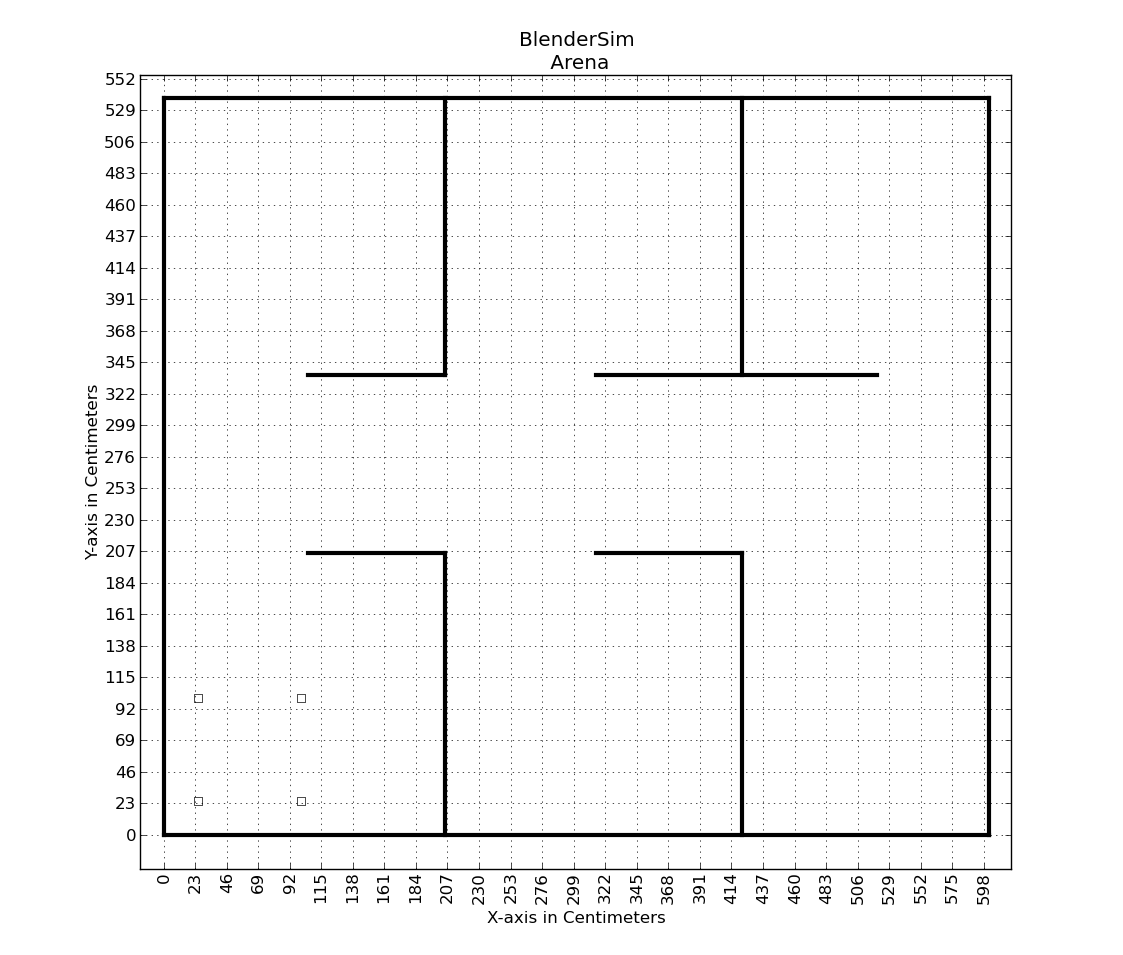
\includegraphics[width=6in]{../Figures/Chapter5/arena.png}
\rule{35em}{0.5pt}
\caption[BlenderSim Arena]{Here you see the layout and dimensions of the arena map both as it is in BlenderSim and in the real HRTeam lab. The smaller four squares in the lower left-hand corner represent the standard starting positions of the robots before any experiment. The grid shown in the plot is the same discrete grid used by HRTeam to calculate the A* generated paths of the robots. }
\label{fig:arena_map}
\end{figure}

\subsection{Surveyor SRV-1 Blackfin 3D Models}

The 3D model of the Surveyor SRV-1 Blackfin is dimensionally and aesthetically representative of its real-life counterpart. The extents of the model are $17.64cm\times14.53cm\times14.33cm$ including the braille hat that rests above the body of the robot. The base and the wheels are the only physics based objects on the model with the wheels being connected to the base via a rigid body hinge joint. See Figure \ref{fig:srv1_3d_model}. Residing $1.37cm$ off the floor from their local origins in the positive z-axis, the robot's base and wheels have their z-translation fixed. The physics parameters governing the wheels are the same highest-fitness parameters found by BBAutoTune in subsection 4.5.1.   

\begin{figure}[htbp]
\centering
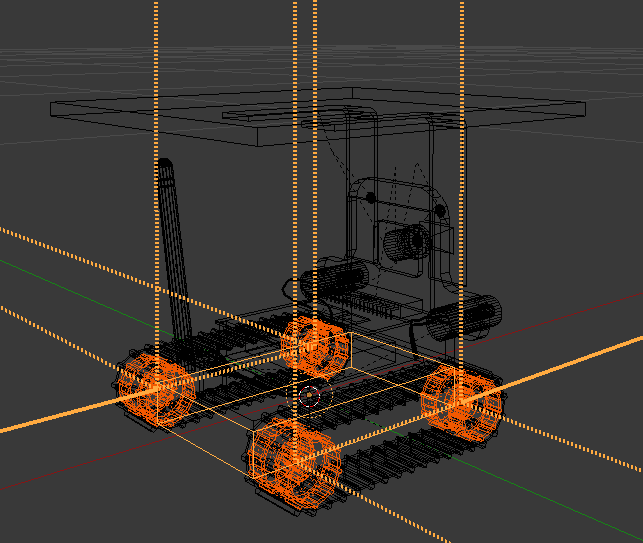
\includegraphics[scale=0.5]{../Figures/Chapter5/srv1.png}
\rule{35em}{0.5pt}
\caption[SRV-1 3D Model]{Here you see the 3D model of the Surveyor SRV-1 Blackfin with the wheels connected to the base via rigid body hinge joints.}
\label{fig:srv1_3d_model}
\end{figure}

% \subsection{Robot Servers}
% 
% \todo{Change this to reflect when BlenderSim communicates directly with HRTeam.}
% 
% The servers are expressed in the simulation as the amber colored \textit{gems} located just above the 3D modeled SRV-1's. See Figure \ref{fig:blendersim_components}. The server logic utilizes the \textit{ServerSocket} Python module. Each of the four servers run in separate threads parented to the Blender process. The four server listen on ports 5001, 5002, 5003 and 5004 respectively. As a connection is made to a client, the server performs a short handshake and begins requesting waypoints from the client. The waypoints are put into a thread safe queue for the robot controller to read from at its leisure. Once the client notifies the server that there are no more waypoints, the server puts \textit{done} in the waypoint queue, sends \textit{done} to the client, shuts down the port, and its thread is terminated.
% 
% If the Blender game engine is terminated before the servers receive all of their waypoints, the servers shut down their ports and their threads are terminated. This allows the simulator to be started again fresh (i.e. \textit{$[$Errno 98$]$ Address already in use.} errors) without having to close Blender itself in order to run another simulation.
% 
% \subsection{Robot Clients}
% 
% \todo{Change this to reflect when BlenderSim communicates directly with HRTeam.}
% 
% The four robot clients connect to ports 5001 through 5004 respectively. Utilizing a custom log reader script, the clients read in their respective waypoints from the waypoint logs. Once connected to their respective servers, the clients perform a short handshake and then begin transmitting waypoints as each of their respective servers request them. Once the clients run out of waypoints to transmit, they signal the servers that there are \textit{nomore} waypoints. Once they receive \textit{done} from their respective server, they close the connection and terminate. Out of convenience, a master script runs the four robot clients in four separate asynchronous sub-processes utilizing the \href{http://docs.python.org/2/library/subprocess.html}{\textit{Subproccess}} Python module.

\subsection{Robot Path Planner}

The robot path planner was greatly simplified for the proof-of-concept. Given a HRTeam experiment log and a robot number, the path planner extracts the A* path points that the real robot was instructed to follow during the HRTeam experiment. This A* path is a path from the robot's starting position to various points of interest or task points. With the path points extracted from the log file, the robot path planner populates the robot controller's waypoint queue. 

\subsection{Robot Controller}

%\todo{Change this to reflect when BlenderSim communicates directly with HRTeam.}

The robot controller is expressed in the simulation as the metal box base of the SRV-1 3D model. See Figure \ref{fig:blendersim_components}. Contained in its logic is a path or waypoint queue that it runs through. This queue is populated by the robot path planner. For each waypoint in the queue, the robot controller will first rotate the robot towards the point and then move the robot forward to reach the point. Once the robot moves forward, the waypoint is removed form the queue. 

For either rotating or moving the robot, the robot controller can only apply torque to the robot's wheels---no other force or mechanism is used to rotate or move the robot. Recalling from subsection 4.5.1 and section 4.6, a torque setting of $82.7271515601$ resulted in the simulated robot moving forward $23.12349975cm$. Since turning had not been learned by BBAutoTune, there were no baseline values of torque versus rotation. To correct for this, the torque value for the robot's left wheels was set to $-20.8$ while the torque value for the right wheels was set to $20.8$ resulting in an in-place rotation of $44.260811$ degrees. 

Using these torque versus displacement values, the robot controller linearly interpolates the amount of torque needed to first rotate the robot towards a waypoint (to within $1$ degree) and then move the robot forward to reach the waypoint. While rotating, if the robot over or undershoots the orientation needed to face the waypoint, the robot controller will continuously interpolate the torque needed to get the robot facing the waypoint to within $1$ degree. Depending on the sign of the angle needed to orient the robot towards the waypoint, the robot controller will either rotate the robot counter-clockwise or clockwise by applying the same magnitude but opposing signs of torque to either the left or right wheels. While move forward, if the robot over or undershoots the position of the waypoint, the robot controller performs no correction but proceeds to orient and move the robot towards the next waypoint in the queue (if there is one). Note that for moving the robot forward, the robot controller applies the same torque value to all four wheels.   

% No robot will move while their respective waypoint queues are empty. Once their waypoint queues begin being populated, by their respective servers, the robots will traverse a linear path to each waypoint first by turning to face the waypoint at a constant velocity and then by moving forward towards the waypoint at a constant linear velocity. The velocities were calculated from a historical physical lab experiment log. Once the robots detect \textit{done} in their waypoint queue, they will cease movement indicating that they have traversed the complete \textit{A*} previously-calculated path as read from the historical physical lab experiment master log.

\subsection{Task Points Manager}

%\todo{Change this to reflect when BlenderSim communicates directly with HRTeam.}

The task points manager is expressed in the simulation as a large torus located above the 3D modeled arena. Once the Blender game engine is started, it hides itself. See Figure \ref{fig:blendersim_components}. At the start of the simulation, the task points manager reads the task points configurations from the task points configuration directory. Controls include keys \textit{\textbf{a}} through \textit{\textbf{e}} where each key corresponds to the five possible task point configurations. See Figure \ref{fig:task_points}. 

\begin{figure}[htbp]
\centering
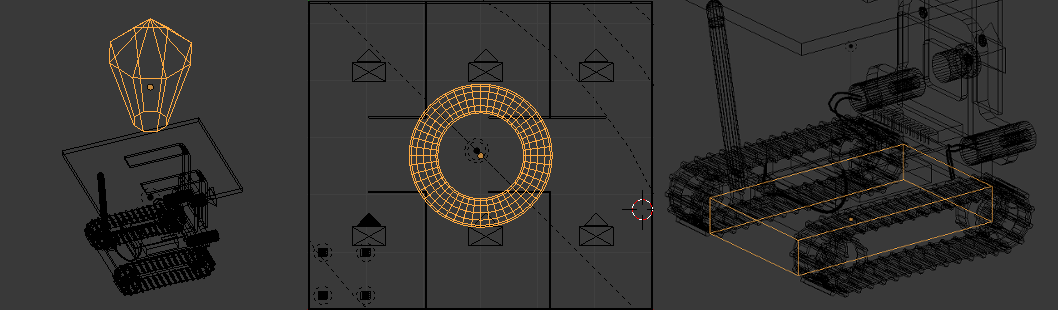
\includegraphics[scale=0.4]{../Figures/Chapter5/parts.png}
\rule{35em}{0.5pt}
\caption[BlenderSim Components]{Here you see from left to right: the robot path planner, the task points manager, and the robot controller manifestations in the simulation.}
\label{fig:blendersim_components}
\end{figure}

\begin{figure}[htbp]
\centering
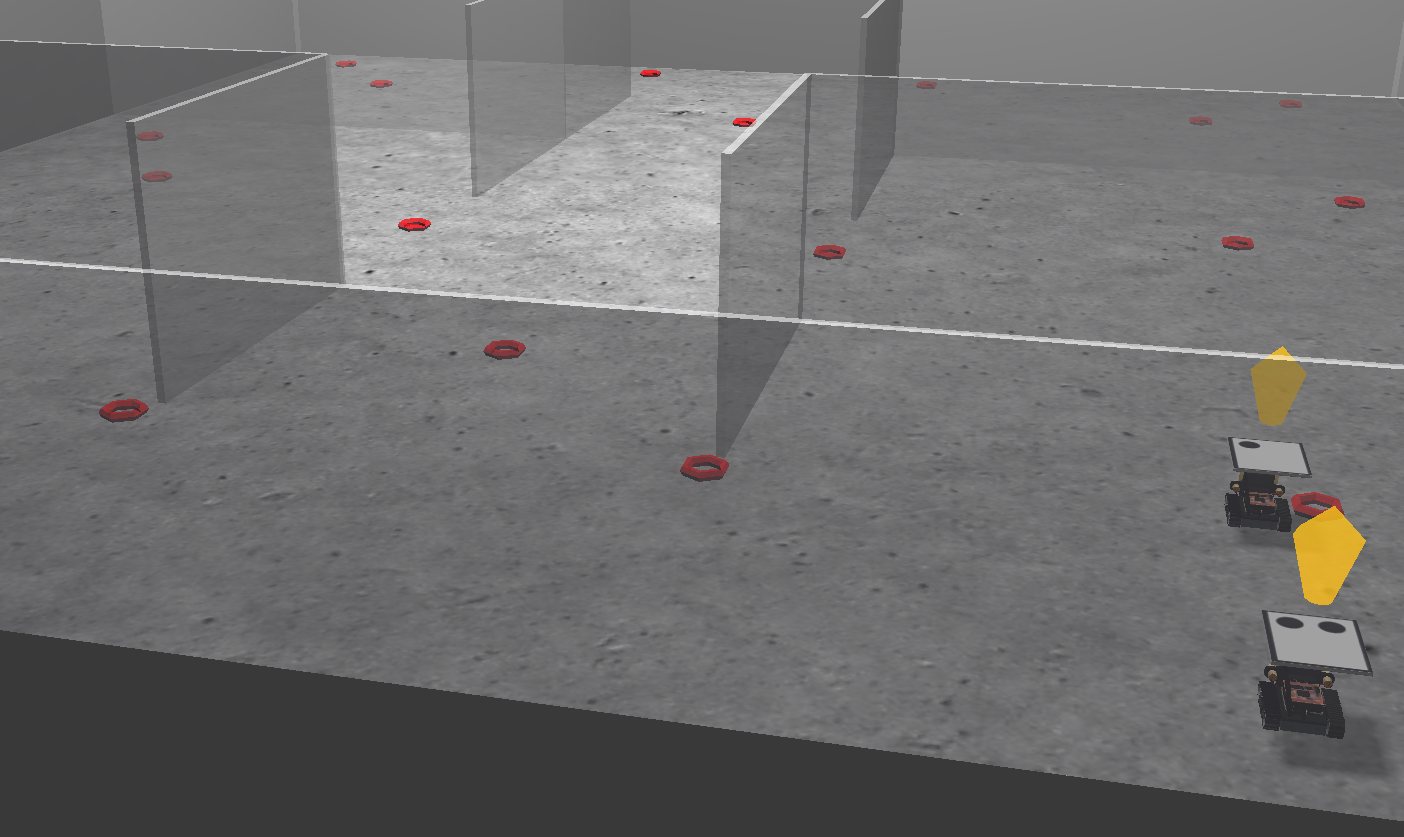
\includegraphics[scale=0.32]{../Figures/Chapter5/taskPoints.png}
\rule{35em}{0.5pt}
\caption[Simulated Task Points]{Here you see the red torus task points laid out in the arena.}
\label{fig:task_points}
\end{figure}

\section{Platform}

BlenderSim was run on a 64bit Linux operating system with 32GB of RAM and an Intel Core i7-4770K four core processor running at 3.9GHz.

\newpage

\section{Experimental Design}

To compare the simulated versus real robot motion (using the physics engine and the highest-fitness physics parameters found by BBAutoTune), a HRTeam experiment was re-run in BlenderSim but for only one robot---specifically robot one with a starting position at $(100cm,100cm)$. The A* path (the waypoints) and the task points that the real robot one was instructed to travel along were extracted from the experiment's log file. Positioning the simulated robot at the same starting position as the real robot in the experiment, the simulated robot was instructed to travel along the same set of waypoints and task points as the real robot was instructed to. See Figure \ref{fig:experiment_arena_layout}.

\begin{figure}[htbp]
\centering
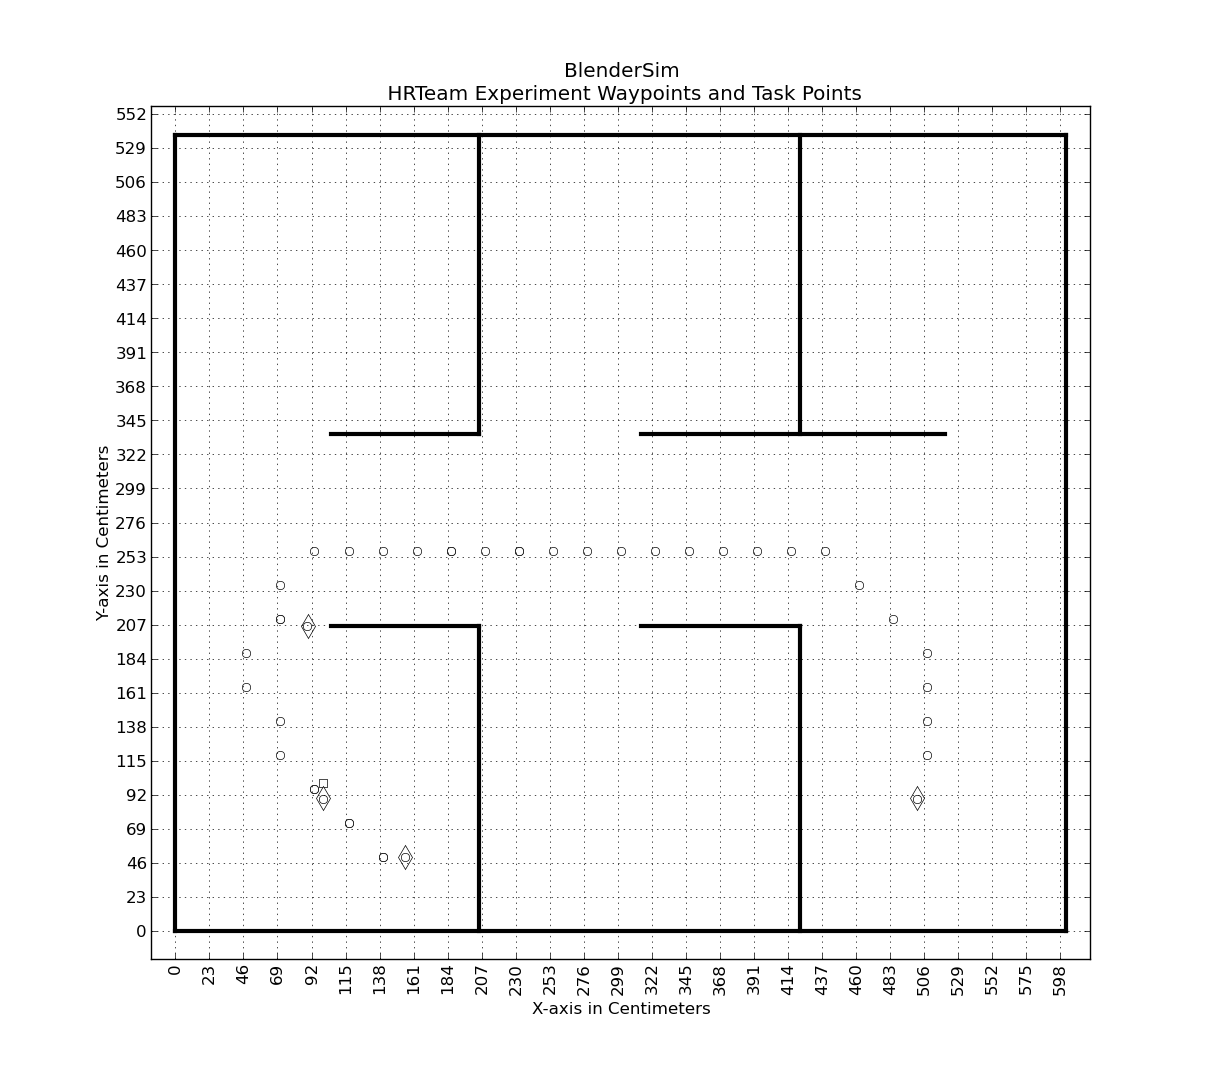
\includegraphics[width=6in]{../Figures/Chapter5/experiment_arena_layout.png}
\rule{35em}{0.5pt}
\caption[HRTeam Experiment Waypoint and Task Points]{Here you see the arena layout with the experiment's waypoints and task points. The white square is the initial position of the robot before the experiment. The white circles are the waypoints and the white diamonds are the task points.}
\label{fig:experiment_arena_layout}
\end{figure}

\newpage

\section{Experimental Result}

Comparing the simulated versus real robot paths, the discrete Fr{\'e}chet and Hausdorff distances between them were $40.575953633cm$ and $19.1208685021cm$ respectively. Between the simulated and real robot paths, the real robot path was the most dissimilar from the waypoint path. See Table \ref{tab:simu_real_fre_dist}, \ref{tab:simu_real_hau_dist}, and Figure \ref{fig:simulated_vs_real_w_physics}.

\begin{table}[htbp]
\centering
\footnotesize
\bgroup
\def\arraystretch{1.1}
\begin{tabular}{ | >{\centering\arraybackslash}m{3cm} | >{\centering\arraybackslash}m{3cm} | >{\centering\arraybackslash}m{3cm} | >{\centering\arraybackslash}m{3cm} | }
%\hline
%\rowcolor{gray}
\cline{2-4}
\multicolumn{1}{c|}{}            & \cellcolor{gray} Simulated & \cellcolor{gray} Real & \cellcolor{gray} Waypoint \\ \hline
\cellcolor{gray} Simulated       & 0.0cm                      & 40.575953633cm        & 16.2376801625cm           \\ \hline
\cellcolor{gray} Real            & 40.575953633cm             & 0.0cm                 & 24.0208242989cm           \\ \hline
\cellcolor{gray} Waypoint        & 16.2376801625cm            & 24.0208242989cm       & 0.0cm                     \\ \hline
\end{tabular}
\egroup
\caption[Simulated vs. Real: Discrete Fr{\'e}chet Distance]{Here you see the discrete Fr{\'e}chet distances between the various paths. }
\label{tab:simu_real_fre_dist}
\end{table}

\begin{table}[htbp]
\centering
\footnotesize
\bgroup
\def\arraystretch{1.1}
\begin{tabular}{ | >{\centering\arraybackslash}m{3cm} | >{\centering\arraybackslash}m{3cm} | >{\centering\arraybackslash}m{3cm} | >{\centering\arraybackslash}m{3cm} | }
%\hline
%\rowcolor{gray}
\cline{2-4}
\multicolumn{1}{c|}{}            & \cellcolor{gray} Simulated & \cellcolor{gray} Real & \cellcolor{gray} Waypoint \\ \hline
\cellcolor{gray} Simulated       & 0.0cm                      & 19.1208685021cm       & 16.2376801625cm           \\ \hline
\cellcolor{gray} Real            & 19.1208685021cm            & 0.0cm                 & 24.0208242989cm           \\ \hline
\cellcolor{gray} Waypoint        & 16.2376801625cm            & 24.0208242989cm       & 0.0cm                     \\ \hline
\end{tabular}
\egroup
\caption[Simulated vs. Real: Hausdorff Distance]{Here you see the Hausdorff distances between the various paths.}
\label{tab:simu_real_hau_dist}
\end{table}

\begin{figure}[htbp]
\centering
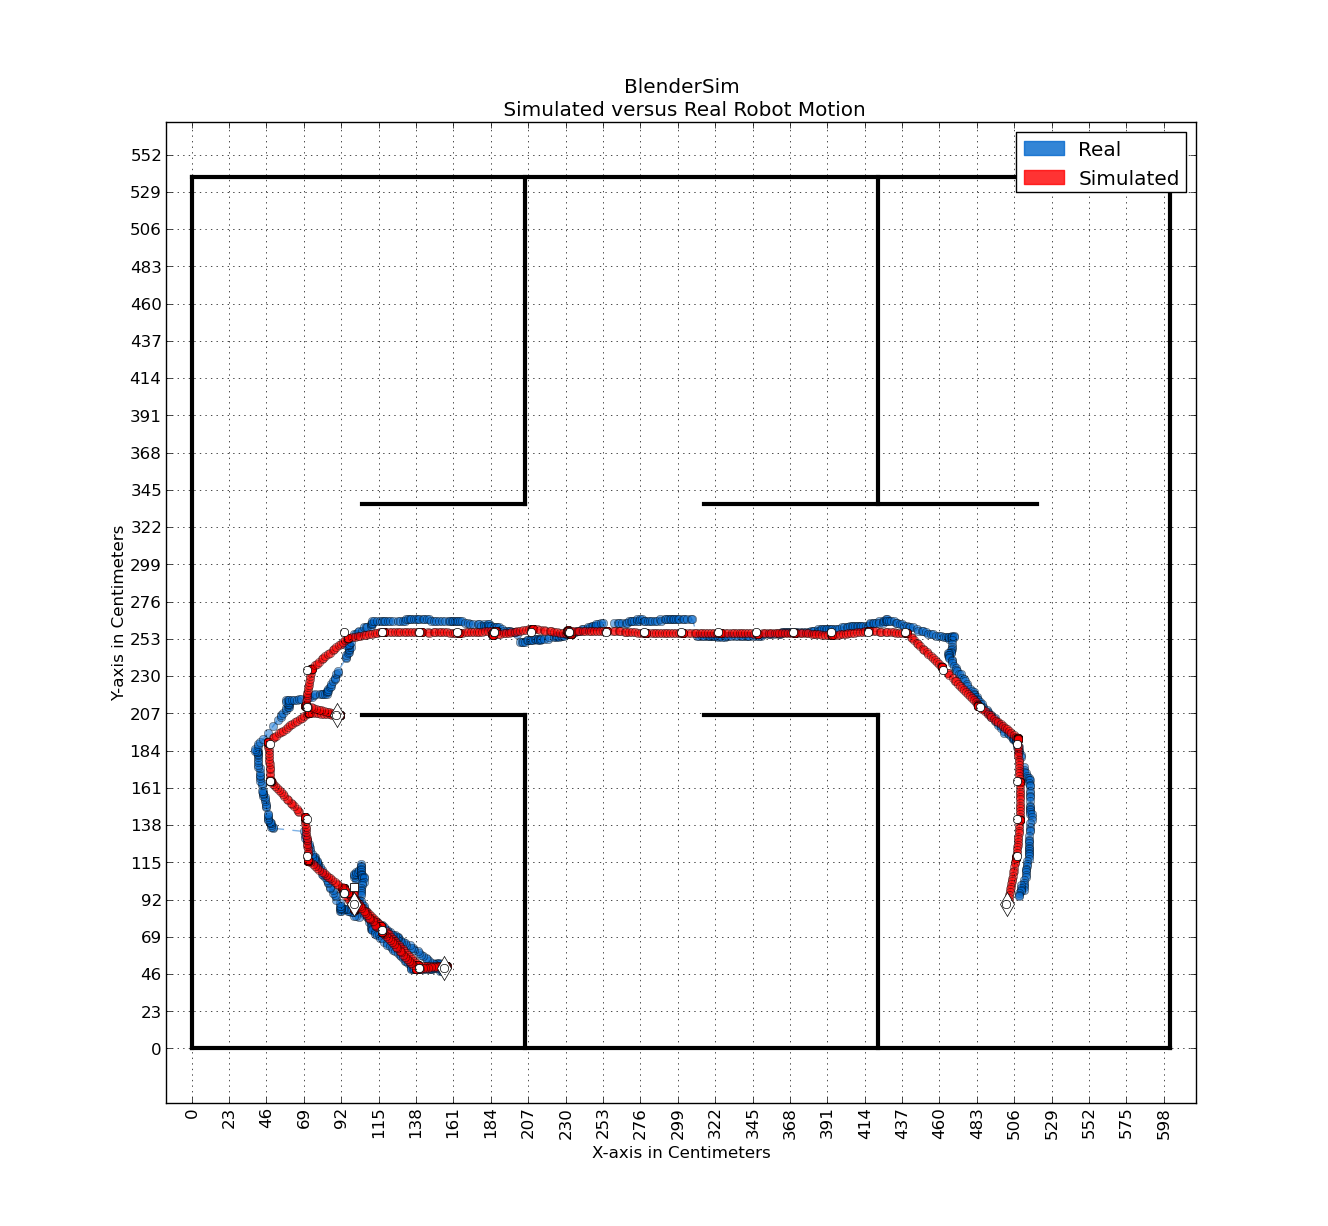
\includegraphics[width=6in]{../Figures/Chapter5/simulated_vs_real_w_physics.png}
\rule{35em}{0.5pt}
\caption[Simulated vs. Real Robot Motion]{Here you see the simulated motion versus the real motion of the robot over the course of the experiment.}
\label{fig:simulated_vs_real_w_physics}
\end{figure}
